\chapauthor{Сердюков Р.Е.\\Зотов Н.В.\\Шункевич Д.В.}
\chapter{Семантическая теория программ для ostis-систем}
\chapauthortoc{Зотов Н.В.\\Шункевич Д.В.}
\label{chapter_programs}

\abstract{Несмотря на активное развитие и использование языков программирования, общей теории программ, на основе которой можно было бы проектировать и разрабатывать прикладные системы на данный момент не существует. В данной главе предлагается единая онтология языков программирования и представления программ на разных языках ппрограммирования. Работа показывает особенности представления программ и ключевые моменты процесса их интерпретации.}


За долгий период развития компьютерных систем (к.с.) практически сняты аппаратные ограничения на решение различных задач. Оставшиеся ограничения отводятся на долю программного обеспечения. Прежде всего эти ограничения связаны с текущими проблемами развития программного обеспечения:
\begin{itemize}
    \item \underline{аппаратная сложность опережает} умение человечества строить \underline{программные к.с.}, использующее потенциальные возможности аппаратуры;
    \item навыки и \underline{технологии} разработки программ \underline{отстают от требований}, предъявлемых к разработке программ нового поколения;
    \item возможностям эксплуатировать существующие программы угрожает \underline{низкое качество их разработки}.
\end{itemize}

Ключом к решению этих проблем является глубокое понимание и грамотное использование существующих языков программирования как основного инструмента для массового создания программных к.с. нового поколения.

В данной главе акцент делается на достижение следующих результатов:
\begin{itemize}
    \item (1) изложить классические основы, отражающие накопленный мировой опыт в области разработки и применения современных языков программирования;
    \item и (2) систематизировать основные результаты в этой области и представить их в виде единой унифицированной семантической теории программ.
\end{itemize}

В данной главе подробно описываются проблемы текущего состояния в области программ и языков программирования. Она посвящена базовым понятиям теории языков программирования, дается обзорная характеристика областей применения языков программирования, достаточно востребованных современным человеческим обществом, рассматриваются способы представления и интерпретации программ различных языков программирования, подробно описываются формы и содержание критериев для оценки эффективности языков.

\section{Проблемы текущего состояния в области разработки и применения языков программирования}

В современную эру развития информационных технологий существует огромное количество языков программирования, каждый из которых имеет своё важное назначение в области проектирования программных систем. Каждый язык демонстрирует не только свою специфику, но имеет свои достоинства и недостатки. Многообразие языков программирования \cite{Sebesta2012} и решений, созданных на них, настолько велико, что очень легко потеряться в море информации о всех аспектах применения и проектирования языков программирования. Кроме этого, основная проблема заключается не в количестве существующих решений в области разработки и применения современных языков программирования, а количестве форм (!), на которых представляются конкретные языки программирования. Так, декларативные знания, то есть знания, являющиеся, например, спецификацией какой-то программы, и процедурные знания, то есть знания, которые являются программами, принадлежащими какому-то языку программирования, представляются совершенно различными способами, методами и средствами.

В связи со сказанным можно выделить следующие ключевые проблемы в области разработки и применения современных языков программирования:
\begin{enumerate}
    \item Поскольку количество языков программирования растёт с увеличением потребности в них, то растут и потребности в описании этих языков программирования для дальнейшего использования и проектирования прикладных систем. Это в свою очередь требует высокого уровня качества спецификации конкретного языка: и описания синтаксиса и семантики конструкций этого языка, и описания средств и методов реновации инструментальных средств, обеспечивающих интерпретацию или трансляцию этого языка. То есть, с увеличением количества языков программирования растёт не только многообразие форм представления знаний (языков программирования), но и количество программных систем на различных формах представления знаний \cite{Zapata2010}.
    \item Большое многообразие форм представления знаний, как говорилось выше, предоставляет большой спектр возможностей проектирования программных к.с. на каждой из них. Получается, чтобы произвести интеграцию нескольких программных систем, реализованных на разных языках программирования, необходимо сделать так, чтобы системы могли коммуницировать между собой на каждом их тех языков, на котором они реализованы \cite{Golenkov2019a}. Так, стремление к использованию существующих программных компонентов затрудняется реализацией самих компонентов, поскольку чтобы объединить эти компоненты необходимо изменить их программный код \cite{Penta2020}, \cite{Scalabrino2016}. Наличие многообразие форм затрудняет реализацию совместимых интероперабельных к.с. \cite{Golenkov2012}.
    \item С ростом сложности программного кода, уменьшается количество способных понять его смысл. Современные разработчики создают программные к.с., не учитывая полный её жизненный цикл \cite{Brooks2021}. Системы должны постоянно обновляться и совершенствоваться с развитием технологий, на которых она основана \cite{Sellitto2022}. Это должно обеспечиваться хорошей документацией реализации компонентов этих систем -- это снижает не только потребности в привлечении новых ресурсов и кадров, но и способствует снижению реинжиниринга программных к.с. \cite{Penta2020}, \cite{Scalabrino2016}.
    \item Полная автоматизация проектирования программных к.с. невозможна, поскольку современные языки, на которых они проектируются не имеют свойства рефлексивности -- системы не могут познавать и понимать себя и развиваться почти в полной мере самостоятельно. Таким образом, существующие интеллектуальные к.с. не являются как таковыми интеллектуальными, потому что не имеют необходимых им свойств \cite{GolenkovPrinciples2021}.
    \item Ключом к легкому и глубокому освоению конкретного языка как основного профессионального инструмента программиста является понимание общих принципов построения и применения языков программирования \cite{Turner2007}, \cite{Constanta2022}, описываемых их общей теорией. До сегодняшнего дня, общей теории языков программирования до сих пор не существует, что затрудняет разработку, верификацию и использование новых и существующих языков программирования. Без общей теории языков программирования каждый может разрабатывать принципиально общие методы и средства так, как хочется, а не так, как требуется \cite{Golenkov2012}.
    \item Достижение максимума услуг и средств при минимуме затрат возможно только путём глубокого понимания принципов построения языков программирования за счёт простоты средств и методов представления знаний. Сложное нужно сводить к простому и изъяснять простыми понятиями, не создавая дополнительной иллюзии важности \cite{Sellitto2022}, \cite{Chaparro2014}, \cite{Posnett2011}.
\end{enumerate}

Все эти проблемы связаны и являются проблемами текущего состояния направлений развития в области Искусственного интеллекта \cite{Skeeter2020}, \cite{Constanta2022}.

Итак, для решения перечисленных проблем необходимо создавать комфортные условия для реализации компьютерных систем, семантически совместимых и интероперабельных между собой. В контексте языков программирования необходима общая теория проектирования программ интеллектуальных к.с. нового поколения, которая:
\begin{enumerate}
    \item \underline{позволит} без больших усилий и затрат \underline{интегрировать имеющиеся решения} в области проектирования программ компьютерных систем \cite{Golenkov2019};
    \item \underline{объединит формы представления знаний} декларативного и процедурного вида;
    \item \underline{будет иметь широкий спектр средств} не только для описания синтаксиса и семантики существующих языков программирования, но и для проектирования новых аналогов;
    \item \underline{будет понятна} не только человеку, но и машине \cite{Zapata2010};
    \item \underline{обозначит принципы}, по которым необходимо проектировать языки программирования нового поколения.
\end{enumerate}

К проектированию таких общих теорий, строго говоря, нужно подходить с высокой степенью важности. Проектируемые к.с. должны всегда иметь возможности использовать те свойства, которые им начертаны. Для того, чтобы и эта теория могла быть использована как некоторая система знаний о том, как надо проектировать и использовать языки программирования и программы в программных к.с., и том, как интерпретировать их программы, необходимо, чтобы эта теория была описана средствами и методами, которыми проектируются эти программные к.с. Речь идёт о том, что принципиально важным подходом к проектированию общей теории программ является онтологический подход \cite{Zapata2010}, \cite{Golenkov2019}, \cite{Sales2022}, \cite{Samaa2020}.

Для воплощения данных идей необходимо изучить и интегрировать опыт, накопленный в области разработки и применения современных языков программирования. Поэтому далее будут рассмотрены результаты других исследований в области проектирования общей теории языков программирования и программ.

\section{Существующие онтологии языков программирования}

В большинстве, идеи, предлагаемые в научных работах по исследованию языков программирования, безусловно являются востребованными и полезными для проектирования программных к.с. Так, идея о том, что языки программирования и программы, реализуемых на них, должны быть организованы в общую таксономию понятий, является основополагающей, поскольку обеспечивает наиболее качественную среду для проектирования и реализации к.с. Общая теория программ нужна не только для того чтобы описывать термины и понятия как некоторую спецификацию, используемую для проектирования программных к.с. (что тоже не мало важно), но и для того, чтобы определять качество языков программирования и программ по таким вопросам, как: \scnqq{Является ли данный язык языком программирования}, \scnqq{Является ли данное знание программой}, \scnqq{Насколько эффективна данная программа}, \scnqq{Какова степень интеллекта данной программной системы} и т. д. Данные идеи предложены и рассмотрены в работах Raymond Turner \cite{Eden2007}, \cite{Turner2012}.

До сегодняшнего дня существует большое количество аналогов онтологий языков программирования и программ. Примеры можно найти в работах \cite{Lando2007}, \cite{Lando2009}, \cite{Turner2007}.  Также стоит отметить разработанные онтологии программ \cite{Turner2012}, \cite{Turner2014}, \cite{Jacobs2022}, система понятий в которых определяется строго и однозначно на формальных языках: языках логики и языках описания грамматик формальных языков. Однако ни одна из них не является таким результатом, который можно было бы использовать при проектировании программных к.с. без существенных проблем. Разработанные онтологии сосредотачивают в себе лишь краткое описание связанных между собой понятий, но общей картины того, как данные онтологии можно использовать в конкретных задачах, почти не видно.

Сегодня встречаются и вовсе протовоположные суждения о назначении программ и языков программирования \cite{Rapaport2020}, противоречающие формальным основам Искусственного интеллекта \cite{Grimmelmann2022}. Программные к.с. должны быть не только понятны человеку, но и сами должны понимать себя, свои возможности, намерения, действия и цели, и понимать себе подобные кибернетические системы. Только таким образом человечество и результаты его деятельности в виде каких-то конкретных систем смогут работать сообща, дополняя друг друга и преумножая свои результаты \cite{Golenkov2012}.

В результате анализа приведенных работ можно сделать вывод о том, что:
\begin{itemize}
    \item общей теории программ и языков программирования, которая могла быть задействована при решении любой прикладной задачи и представлении и реализации средств проектирования компьютерных систем до сих пор не сложилась;
    \item унификация представления средств описания и реализации по этим описании как главный аргумент к оперированию смысловому представлению знаний, к полному взаимопониманию между компьютерными системы вовсе не рассматривается;
    \item программы и совокупности этих программ в виде программных к.с. реализуются в большинстве случаев в индивидуальном порядке и плохо документируются, что усложняет их использование, интеграцию с другими программами и программными к.с., тестирование и совершенствование.
\end{itemize}

Ключом к решению всех этих проблем является общая технология проектирования компьютерных систем нового поколения, на базе которой можно построить общую теорию программ (дисциплину программирования) \cite{Deikstra1978}, которая будет рассмотрена дальше.

\section{Предлагаемое решение}

Несмотря на обширное разнобразие используемых человечеством классических технологий, общего решения, позволяющего решить поставленну проблему в комплексе, не существует.

Почему Технология OSTIS является ключом к решению описанных проблем?
\begin{enumerate}
    \item {Стандарт Технологии OSTIS \cite{Standard2021} уже в меньшей мере реализует базовые средства, необходимые для проектирования и разработки интероперабельных к.с., в основе которых лежит смысловое представление знаний. Это устраняет не только необходимость создания онтологий верхнего уровня, которые должны быть использованы в общей теории программ как базовые для описания понятий этой теории, но и помогает проектировать решения согласованно с другими онтологиями. В результате формируется общая слаженная картина мира, которая (1) непротиворечива, то есть согласована, (2) однозначно трактуема, (3) универсальная и, (4) самое главное, понятна для каждого.}
    \item {Технология OSTIS проектируется одним языком унифицированного представления знаний, называемым SC-кодом. Смысл программ и языков программирования понятен и однозначен тогда и только тогда, когда этот смысл описывается на одном общем языке, понятному любой кибернетической системе.}
    \item {SC-код синтаксически минимален. Для описания объектов и связей между ними используется минимальное количество знаков. В то же время многообразие этих связей сводится к многобразию знаковых конструкций. Всё это обеспечивается за счёт представления информации в виде графовых структур \cite{Kasyanov2003}, \cite{Petrov1978}.}
    \item {SC-код не просто удобен для описания и проектирования каких-то сложных объектов -- с его помощью можно проектировать и реализовывать любые языки представления знаний, в том числе программ, компьютерные системы и, вообще, реальный мир.}
    \item {Онтологический и компонентный подходы \cite{Sales2022}, \cite{Samaa2020} к проектированию любых сложных объектов обеспечивают выполнение главных принципов, по которым должны проектироваться современные системы. То, что реализовано и можно использовать, нужно переиспользовать везде \cite{O4IS2007}, \cite{Molorodov2019}.}
\end{enumerate}

Таким образом, решением всех проблем будет являться общая теория программ, трактуемая как онтология общей системы, реализуемой посредством Технологии OSTIS.

\section{Общее описание проектируемых предметных областей и онтологий}

Результатом данной работы является \textit{Предметная область и онтология методов} (Предметная область и онтология программ), с помощью которой можно задавать методы (программы), их синтаксис, денотационную и операционную семантику. \textit{Предметная область и онтология методов} является дочерней предметной областью по отношению к \textit{Предметной области и онтологии информационных конструкций и языков}. Это означает, что она наследует все свойства исследуемых в ней понятий и отношений.

\begin{SCn}
\scnheader{Предметная область и онтология информационных конструкций и языков}
\begin{scnrelfromlist}{дочерняя предметная область}
    \scnitem{Предметная область и онтология языков}
    \begin{scnindent}
        \begin{scnrelfromlist}{дочерняя предметная область}
            \scnitem{Предметная область и онтология естественных языков}
            \scnitem{Предметная область и онтология формальных языков}
        \end{scnrelfromlist}
    \end{scnindent}
\end{scnrelfromlist}
\end{SCn}

\begin{SCn}
\scnheader{Предметная область и онтология формальных языков}
\begin{scnrelfromlist}{дочерняя предметная область}
    \scnitem{Предметная область и онтология языков представления знаний}
    \begin{scnindent}
        \begin{scnrelfromlist}{дочерняя предметная область}
            \scnitem{\scnkeyword{Предметная область и онтология методов}}
        \end{scnrelfromlist}
    \end{scnindent}
\end{scnrelfromlist}
\end{SCn}

\begin{SCn}
\scnheader{Предметная область и онтология методов}
\begin{scnrelfromlist}{дочерняя предметная область}
    \scnitem{Предметная область и онтология методов ostis-систем}
    \begin{scnindent}
        \begin{scnrelfromlist}{дочерняя предметная область}
            \scnitem{Предметная область и онтология процедурных методов ostis-систем}
        \end{scnrelfromlist}
    \end{scnindent}
\end{scnrelfromlist}
%%%% описать классы и отношения
\end{SCn}

\section{Понятие метода (программы)}

Каждая теория должна быть согласована понятийно. Несмотря на то, что в литературе сложилась разное трактование понятия языка программирования, должно быть одно универсальное. Для этого вместо языков программирования далее \underline{будем говорить о языках представления методов}, а вместо программ этих языков программирования -- о методах как знаковых конструкциях языков представления методов (я.п.м.). Такое решение обосновывается тем, что обычно язык выступает в роли инструмента какого-то знания определенного вида, а термин языка программирования является вырожденным, поскольку стоит говорить не о языках, на которых что-то можно программировать, а о языках, на которых можно представлять знания определённого вида, в данном случае -- знания процедурного вида. Сами термины \scnqqi{языка программирования} и \scnqqi{программы} будем считать неосновными идентификаторами понятий \scnqqi{языка представления методов} и \scnqqi{метода}, соответственно.

Формально, \textit{метод} -- это спецификация решения задачи какого-то класса \cite{Standard2021}, \cite{Tuzov1986}. В состав спецификации каждого класса задач входит описание способа \scnqq{привязки} метода к исходным данным конкретной задачи, решаемой с помощью этого метода.

\begin{SCn}
\scnheader{метод}
\scnidtf{программа}
\scnidtf{описание того, как может быть выполнено любое или почти любое действие, принадлежащее соответствующему классу действий}
\scnidtf{метод решения соответствующего класса задач, обеспечивающий решение любой или большинства задач
указанного класса}
\scnidtf{обобщенная спецификация решения задач соответствующего класса}
\scnidtf{программа решения задач соответствующего класса, которая может быть как процедурной, так и декларативной (непроцедурной)}
\scnidtf{знание о том, как можно решать задачи соответствующего класса}
\scnsubset{знание}
\scniselement{вид знаний}
\scnidtf{способ}
\scnsuperset{модель решения задач}
\end{SCn}

\section{Понятие класса методов. Общая классификация методов}

Иногда целесообразным может считаться выделение некоторого подмножества методов (например, множества методов, с помощью которых решается определённая задача), тогда в таком случае для этих методов можно описать требования, которые они должны выполнять. Такие множества методов являются \textit{классами методов} некоторого я.п.м., которым ставится в соответствие конкретная \textit{модель решения задач}. Методы могут быть как \textit{процедурные}, так и \textit{непроцедурные} \cite{Turner2007}.

\begin{SCn}
\scnheader{класс методов}
\scnrelto{семейство подклассов}{метод}
\scnidtf{множество методов, для которых можно унифицировать представление (спецификацию) этих методов}
\scnidtf{множество всевозможных методов решения задач, имеющих общий язык представления этих методов}
\scnidtf{множество методов, для которых задан язык представления этих методов}
\scnhaselement{процедурный метод решения задач}
\begin{scnindent}
    \scnsuperset{алгоритмический метод решения задач}
\end{scnindent}
\scnhaselement{непроцедурный метод решения задач}
\begin{scnindent}
    \scnsuperset{логический метод решения задач}
    \scnsuperset{продукционный метод решения задач}
    \scnsuperset{функциональный метод решения задач}
    \begin{scnindent}
        \scnsuperset{искусственная нейронная сеть}
        \scnsuperset{генетический \scnqq{алгоритм}}
    \end{scnindent}
\end{scnindent}
\scnidtf{множество методов, которому ставится в соответствие отдельная модель решения задач}
\end{SCn}

Поскольку каждому методу соответствует обобщенная формулировка задач, решаемых с помощью этого метода, то каждому классу методов должен соответствовать не только определенный я.п.м, принадлежащих указанному \textit{классу методов}, но и определенный язык представления обобщенных формулировок задач для различных классов задач, решаемых с помощью методов, принадлежащих указанному классу методов.

Для процедурных и непроцедурных методов хоть и можно задать \textit{входные} и \textit{выходные параметры}, но нельзя задать общую денотационную семантику их логических элементов: для процедурных методов -- это операторы, для непроцедурных -- математические объекты предметной области.

\section{Понятие языка представления методов (языка программирования)}

Каждому конкретному классу методов взаимно однозначно соответствует я.п.м., принадлежащих этому (специфицируемому) классу методов. Таким образом, спецификация каждого класса методов сводится к спецификации соответствующего я.п.м., т.е. к описанию его синтаксической, денотационной семантики и операционной семантики. Примерами я.п.м. являются все языки программирования, которые в основном относятся к подклассу я.п.м. Но сейчас все большую актуальность приобретает необходимость создания эффективных формальных я.п.м. выполнения действий во внешней среде кибернетических систем. Без этого комплексная автоматизация \cite{Pospelov2021}, в частности, в промышленной сфере невозможна.

Под \textit{языком представления методов} будем подразумевать формальный язык, (1) знаковыми конструкциями которого являются соответствующие методы, для которых существуют общие правила построения и (2) общие правила соотнесения с теми сущностями и связями между ними, которые описываются этими методами.

С помощью я.п.м. формируются \textit{сообщения} (методы) для компьютера. Эти сообщения должны быть понятны (семантически корректны и целостны) компьютеру.

\begin{SCn}
\scnheader{язык представления методов}
\scnidtf{язык программирования}
\scnsubset{язык представления знаний}
\begin{scnindent}
    \scnsubset{формальный язык}
\end{scnindent}
\scnidtf{компьютерный язык}
\scnidtf{формальный язык, (1) знаковыми конструкциями которого являются соответствующие методы, для которых существуют общие правила построения и (2) общие правила соотнесения с теми сущностями и связями между ними, которые описываются этими методами}
\scnidtf{средство общения между человеком (пользователем) и компьютером (исполнителем)}
\scnidtf{инструмент для производства программных услуг}
\end{SCn}

Метод принадлежит языку представления методов, если он является синтаксически корректным, синтаксически целостным, семантически корректным и семантически целостным методом заданного я.п.м. (!).

\begin{SCn}
\scnheader{отношение, заданное на множестве языков представления методов\scnsupergroupsign}
\scnidtf{отношение, область определения которого включает в себя множество всевозможных языков представления методов}
\scnhaselement{метод заданного языка представления методов*}
\scnhaselement{синтаксически корректный метод для заданного языка представления методов*}
\begin{scnindent}
    \scnidtf{метод, не содержащий синтаксических ошибок для заданного языка представления методов*}
    \scnsubset{синтаксически корректная знаковая конструкция для заданного языка*}
\end{scnindent}
\scnhaselement{синтаксически целостный метод для заданного языка представления методов*}
\begin{scnindent}
    \scnsubset{синтаксически целостная знаковая конструкция для заданного языка*}
\end{scnindent}
\scnhaselement{семантически корректный метод для заданного языка представления методов*}
\begin{scnindent}
    \scnidtf{метод, не содержащий семантических ошибок для заданного языка представления методов*}
    \scnsubset{семантически корректная знаковая конструкция для заданного языка*}
\end{scnindent}
\scnhaselement{семантически целостный метод для заданного языка представления методов*}
\begin{scnindent}
    \scnsubset{семантически целостная знаковая конструкция для заданного языка*}
    \scnidtf{метод заданного языка представления методов, содержащий достаточную информацию для установления его
    истинности*}
\end{scnindent}
\end{SCn}

\begin{SCn}
\scnheader{метод заданного языка представления методов*}
\scnidtf{метод, принадлежащий заданному языку программирования*}
\scnsubset{текст заданного языка*}
\scnrelfrom{второй домен}{метод}
\begin{scnreltoset}{объединение}
    \scnitem{\scnnonamednode}
    \begin{scnindent}
        \begin{scnreltoset}{объединение}
            \scnitem{синтаксически корректный метод для заданного языка представления методов*}
            \scnitem{синтаксически целостный метод для заданного языка представления методов*}
        \end{scnreltoset}
    \end{scnindent}
    \scnitem{\scnnonamednode}
    \begin{scnindent}
        \begin{scnreltoset}{объединение}
            \scnitem{семантически корректный метод для заданного языка представления методов*}
            \scnitem{синтаксически целостный метод для заданного языка представления методов*}
        \end{scnreltoset}
    \end{scnindent}
\end{scnreltoset}
\end{SCn}

\section{Общая классификация языков представления методов}

Языки представления методов в современном информационном обществе различают по их парадигмам: \textit{процедурные}, \textit{функциональные}, \textit{логические}, \textit{объектно-ориентированные} и т. д. Таким, например, в методах процедурного я.п.м. решение задачи компьютером формируется в виде последовательности операторов, в методах функционального я.п.м. — указанием других методов. В логическом я.п.м. применяются высказывания, а в объектно-ориентированном — объекты.

\begin{SCn}
\scnheader{язык представления методов}
\scnsuperset{язык представления методов общего назначения}
\begin{scnindent}
    \scnidtf{язык программирования общего назначения}
\end{scnindent}
\scnsuperset{предметно-ориентированный язык представления методов}
\begin{scnindent}
    \scnidtf{предметно-ориентированный язык программирования}
\end{scnindent}
\scnrelfrom{разбиение}{парадигма языка представления методов\scnsupergroupsign}
\begin{scnindent}
    \begin{scneqtoset}
        \scnitem{процедурный язык представления методов}
        \scnitem{непроцедурный язык представления методов}
    \end{scneqtoset}
\end{scnindent}
\end{SCn}

\textit{Процедурные языки представления методов} задают вычисления как последовательность операторов (команд).
Они ориентированы на компьютеры с архитектурой фон Неймана. Основные понятия процедурных я.п.м. тесно связаны с компонентами компьютера:
\begin{itemize}
    \item переменными различных типов, которые моделируют ячейки памяти компьютера;
    \item операторами присваивания, которые моделируют пересылки данных между участками памяти;
    \item повторений действий в форме итерации, которые моделируют хранение информации в смежных ячейках памяти;
    \item и другое.
\end{itemize}

\begin{SCn}
\scnheader{процедурный язык представления методов}
\scnidtf{императивный язык представления методов}
\scnsuperset{структурный язык представления методов}
\begin{scnindent}
    \begin{scnhaselementrolelist}{пример}
        \scnitem{Fortran}
        \scnitem{Си}
        \scnitem{Pascal}
    \end{scnhaselementrolelist}
\end{scnindent}
\scnsuperset{объектно-ориентированный язык представления методов}
\begin{scnindent}
    \begin{scnhaselementrolelist}{пример}
    	\scnitem{Java}
        \scnitem{Smalltalk}
        \scnitem{HTML}
    \end{scnhaselementrolelist}
    \scnsuperset{аспектно-ориентированный язык представления методов}
\end{scnindent}
\scnsuperset{скриптовый язык представления методов}
\begin{scnindent}
    \scnidtf{склеивающий язык представления методов}
\end{scnindent}
\end{SCn}

\textit{Непроцедурные языки представления методов}, в отличие от процедурных, задают вычисления как последовательность связанных между собой объектов. Основные понятия непроцедурных я.п.м. обычно не связаны с компонентами компьютера.

\begin{SCn}
\scnheader{непроцедурный язык представления методов}
\scnidtf{декларативный язык представления методов}
\scnsuperset{логический язык представления методов}
\begin{scnindent}
    \begin{scnhaselementrolelist}{пример}
        \scnitem{Prolog}
    \end{scnhaselementrolelist}
\end{scnindent}
\scnsuperset{продукционный язык представления методов}
\scnsuperset{функциональный язык представления методов}
\begin{scnindent}
    \scnidtf{аппликативный язык представления методов}
    \begin{scnhaselementrolelist}{пример}
        \scnitem{LISP}
    \end{scnhaselementrolelist}
\end{scnindent}
\end{SCn}

\section{Представление синтаксиса и семантики различных методов}

\textit{Синтаксис} и \textit{семантика} метода представляют его \textit{спецификацию}. Семантику метода можно рассматривать с двух ракурсов: как множество знание, связанных между собой, что определяется денотационной семантикой данного метода, и как знание, которое может быть проинтерпретировано другим методом, что определяется операционной семантикой данного метода.

\begin{SCn}
\scnheader{спецификация метода*}
\begin{scnrelfromset}{разбиение}
    \scnitem{синтаксис метода*}
    \scnitem{денотационная семантика метода*}
    \begin{scnindent}
        \scnidtf{обобщенная формулировка класса задач, решаемых с помощью данного метода*}
        \scnrelboth{семантически близкий знак}{обобщенная формулировка задач соответствующего класса методов*}
    \end{scnindent}
    \scnitem{операционная семантика метода*}
    \begin{scnindent}
        \scnidtf{перечень обобщенных агентов, обеспечивающих интерпретацию метода*}
        \scnidtf{семейство методов интерпретации данного метода*}
        \scnidtf{формальное описание интерпретатора заданного метода*}
    \end{scnindent}
\end{scnrelfromset}
\end{SCn}

\subsection{Представление синтаксиса метода решения задачи}

Любый метод состоит из атомарных информационных конструкций, которые задают порядок действий в базе знаний, с помощью которых нужно перейти от исходного состояния к \underline{целевому}, решив таким образом какую-то конкретную задачу. Так, например, в процедурном методе любой такой оператор представляет собой некоторую математическую функцию. Для композиции этих функций в более крупные фрагменты используются выражения и операторы. В свою очередь, линейные последовательности операторов и условные ветвления также могут быть представлены функциями, составленными из функций отдельных компонентов этих конструкций. Цикл легко описывается рекурсивной функцией, составленной из компонентов, входящих в его тело.

\textit{Синтаксис метода*} определяет множество его допустимых конструкций. Внешний вид элементо метода задают с помощью конкретного синтаксиса. Он описывает такие лексические детали, как размещение ключевых слов и знаков пунктуации. Для спецификации конкретного синтаксиса применяют грамматики.

Синтаксис я.п.м. в ostis-системах может быть формально описан различными способами. Так, например, можно использовать метаязык Бэкуса-Наура для описания синтаксиса какого-то методов конкретного я.п.м. Другими не менее известными формами представления методов являются контекстно-свободные грамматики, расширенная форма Бэкуса-Наура, синтаксические графы \cite{Sebesta2012}, \cite{Scott2006}, \cite{Scott1972}.

Однако значительно более логично и целесообразно описывать синтаксис других языков на универсальном языке представления знаний -- \textit{SC-коде}. Такой подход позволит ostis-системам самостоятельно понимать, анализировать и генерировать тексты указанных языков на основе принципов, общих для любых форм внешнего представления информации, в том числе нелинейных \cite{Petrov1978}. Таким образом, языки, написанные на SC-код, имеют такой же синтаксис как и сам SC-код.

\subsection{Представление денотационной семантики метода}

Семантика метода разъясняет смысл синтаксических конструкций метода. Наиболее распространенными методами описания семантики языков программирования являются: денотационный, операционный, аксиоматический, алгебраический \cite{Orlov2013}. На базе принципов Технологии OSTIS, под семантикой метода будем подразумевать объединение денотационной и операционной семантик метода.

Описание способа \scnqq{привязки} метода к какому-то классу задач включает в себя:
\begin{itemize}
    \item набор переменных, которые входят как в состав метода, так и в состав обобщенной формулировки задач соответствующего класса, и значениями которых являются соответствующие элементы исходных данных каждой конкретной решаемой задачи;
    \item часть обобщенной формулировки задач того класса, которому соответствует рассматриваемый метод, являющихся описанием условия применения этого метода;
    \item описание условаия инициирования метода и его результа;
    \item описание начальной и целевой ситуаций в sc-памяти.
\end{itemize}

\scnqq{Привязка} метода к конкретной задаче, решаемой с помощью этого метода осуществляется путем поиска в базе знаний такого фрагмента, который удовлетворяет условиям применения указанного метода. Одним из результатов такого поиска и является установление соответствия между указанными выше переменными используемого метода и значениями этих переменных в рамках конкретной решаемой задачи. Другим вариантом установления рассматриваемого соответствия является явное обращение (вызов, call) соответствующего метода (программы) с явной передачей соответствующих параметров. Но такое не всегда возможно, т.к. при выполнении процесса решения конкретной задачи на основе декларативной спецификации выполнения этого действия нет возможности установить:
\begin{itemize}
    \item когда необходимо инициировать вызов (использование) требуемого метода;
    \item какой конкретно метод необходимо использовать;
    \item какие параметры, соответствующие конкретной инициируемой задаче, необходимо передать для \scnqq{привязки} используемого метода к этой задаче.
\end{itemize}

Под \textit{процессом} понимается некоторое действие в sc-памяти, однозначно описывающее конкретный акт выполнения некоторого метода для заданных исходных данных \cite{Deikstra1978}. Если метод описывает алгоритм решения какой-либо задачи в общем виде, то процесс обозначает конкретное действие, реализующее данный алгоритм для заданных входных параметров. По сути, процесс представляет собой уникальную копию, созданную на основе метода, в котором каждой sc-переменной, соответствует сгенерированная sc-константа.

\begin{SCn}
\scnheader{отношение, заданное на множестве (процесс)\scnsupergroupsign}
\scnidtf{отношение, область определения которого включает в себя множество всевозможных процессов}
\scnhaselement{параметр'}
\begin{scnrelfromset}{разбиение}
    \scnitem{in-параметр'}
    \scnitem{out-параметр'}
\end{scnrelfromset}
\scnhaselement{in-параметр'}
\scnhaselement{out-параметр'}
\scnhaselement{начальная информационная конструкция'}
\scnhaselement{подпроцесс*}
\end{SCn}

Процесс \scnqq{привязки} метода решения задач к конкретной задаче, решаемой с помощью этого метода, можно также представить как процесс, состоящий из следующих этапов:
\begin{itemize}
    \item построение копии используемого метода;
    \item склеивание основных (ключевых) переменных используемого метода с основными параметрами конкретной решаемой задачи.
\end{itemize}

В результате этого на основе рассматриваемого метода используемого в качестве образца (шаблона) строится спецификация процесса решения конкретной задачи. Описание процесса \scnqq{привязки} метода решения к конкретной задаче, а также описание элементов метода является \textit{денотационной семантикой данного метода}.

\begin{SCn}
\scnheader{денотационная семантика метода}
\scnhaselement{общая формулировка класса задач*}
\begin{scnindent}
    \scnidtf{текстовая формулировка множества задач, решаемых данным методом}
    \scnsubset{пояснение*}
\end{scnindent}
\scnhaselement{первичное условие инициирования*}
\scnhaselement{условие инициирования и результат*}
\begin{scnindent}
    \begin{scnreltovector}{декартово произведение}
        \scnitem{класс методов}
        \scnitem{импликация*}
    \end{scnreltovector}
\end{scnindent}
\scnhaselement{условие начальной и целевой ситуаций*}
\begin{scnindent}
    \begin{scnreltovector}{декартово произведение}
        \scnitem{класс методов}
        \scnitem{импликация*}
    \end{scnreltovector}
\end{scnindent}
\end{SCn}

Пример части спецификации, описывающей денотационную семантику Метода нахожденя удвоенной суммы двух чисел, приведён на рисунке \ref{fig:condition_and_result}.

\begin{figure}[htbp]
  \center
  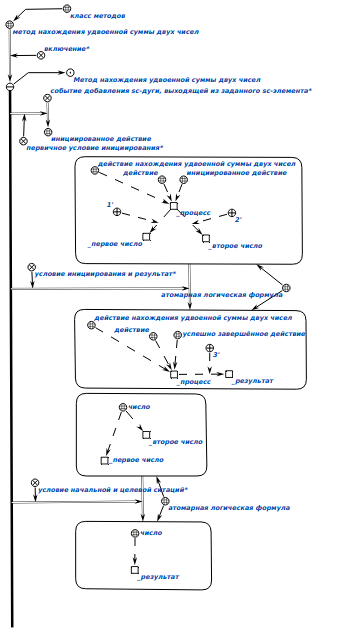
\includegraphics[scale=0.6]{author/part3/figures/condition_and_result.png}
  \caption{Спецификация метода решения задачи вычисления удвоенной суммы двух чисел}
  \label{fig:condition_and_result}
\end{figure}

Отношение \textit{общая формулировка класса задач*} представляет собой класс sc-связок между sc-связкой, обозначающей множество методов, и файлом ostis-системы, являющийся пояснением того, какие классы задач можно решать при помощи данного множества методов. В некоторых редких случаях наличие такой sc-связки в спецификации метода может и не быть, поскольку нет необходимости уточнять, какие классы задач можно решать при помощи данного метода.

Связки отношения \textit{первичное условие инициирования*} связывают между собой sc-связку, обозначающий множество методов, и бинарную ориентированную пару, описывающую первичное условие инициирования данного метода, т.е. такой спецификацию ситуации в sc-памяти, возникновение которой побуждает метаметод-исполнитель перевести заданное множество методов в активное состояние и начать проверку наличия их полного условия инициирования.

Первым компонентом данной ориентированной пары является знак некоторого класса элементарных событий в sc-памяти*, например, событие добавления sc-дуги, выходящей из заданного sc-элемента*.

Вторым компонентом данной ориентированной пары является произвольный в общем случае sc-элемент, с которым непосредственно связан указанный тип события в sc-памяти, т.е., например, sc-элемент, из которого выходит либо в который входит генерируемая либо удаляемая sc-дуга, либо файл, содержимое которого было изменено.

Связки отношения \textit{условие инициирования и результат*} связывают между собой sc-связку, обозначающий множество методов, и бинарную ориентированную пару, связывающую условие инициирования данного множества методов и результаты выполнения этого множества методов в какой-либо конкретной системе. Указанную ориентированную пару можно рассматривать как логическую связку импликации, при этом на sc-переменные, присутствующие в обеих частях связки, неявно накладывается квантор всеобщности, на
sc-переменные, присутствующие либо только в посылке, либо только в заключении неявно накладывается
квантор существования.

Первым компонентом указанной ориентированной пары является логическая формула, описывающая условие инициирования описываемого метода, то есть конструкции, наличие которой в sc-памяти вызывает множество методов для началы работы по изменению состояния в sc-памяти. Данная логическая формула может быть как атомарной, так и неатомарной, в которой допускается использование любых связок логического языка.

Вторым компонентом указанной ориентированной пары является логическая формула, описывающая возможные результаты выполнения описываемого множества методов, то есть описание произведенных им изменений состояния sc-памяти. Данная логическая формула может быть как атомарной, так и неатомарной, в которой допускается использование любых связок логического языка.

Связки отношения \textit{условие начальной и целевой ситуации*} связывают между собой sc-связку, обозначающий множество методов, и бинарную ориентированную пару, связывающую начальную и целевую ситуации в sc-памяти, то есть, кратко говоря, ситуацию до применения метода и желаемую ситуацию после применения метода. Указанную ориентированную пару можно также рассматривать как логическую связку импликации, при этом на sc-переменные, присутствующие в обеих частях связки, неявно накладывается квантор всеобщности, на sc-переменные, присутствующие либо только в посылке, либо только в заключении неявно накладывается квантор существования. Для первой и второй копненты указанной ориентированной пары накладывается те же ограничения и свойства, что для компонент ориентированной пары, являющейся вторым компонентом отношения \textit{условие инициирования и результат*}.

Стоит отметить, что связки отношения \textit{условие инициирования и результат*} и отношения \textit{условие начальной и целевой ситуации*} могут быть представлены иначе. Иногда может и не быть необходимости создавать и проверять второе условие метода, по которому проверяется наличие начальной ситуации в sc-памяти и проверка достижения целевой ситуации в sc-памяти в результате применения метода. Если так, то условие начальной и целевой ситуации* может быть уточнено в логическах формулах, являющихся компонентами второго компонента связки отношения \textit{условие инициирования и результат*}.

Программы в зависимости от его способа задания в конкретном языке представления методов будут различаться. В этом можно убедиться, сравнив примеры процедурного (рис. \ref{fig:procedural_program}) и логического (рис. \ref{fig:logic_program}) методов решения одной и той же задачи.

\begin{figure}[htbp]  
  \center
  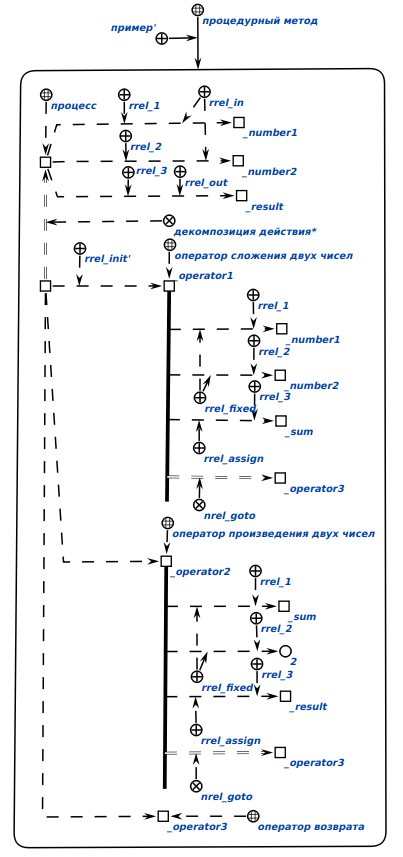
\includegraphics[scale=0.6]{author/part3/figures/procedural_program.png}
  \caption{Пример процедурного метода решения задачи вычисления удвоенной суммы двух чисел}
  \label{fig:procedural_program}
\end{figure}

\begin{figure}[htbp]
  \center
  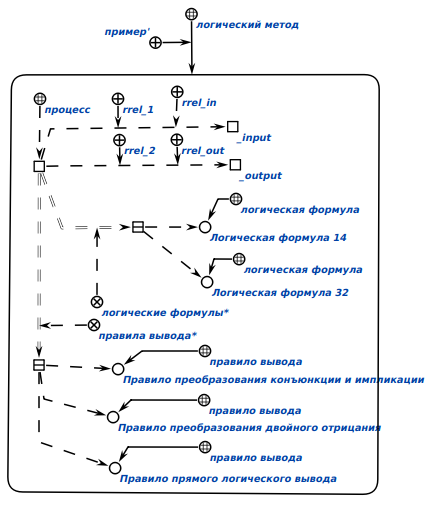
\includegraphics[scale=0.6]{author/part3/figures/logic_program.png}
  \caption{Пример логического метода решения задачи вычисления удвоенной суммы двух чисел}
  \label{fig:logic_program}
\end{figure}

С помощью SC-кода можно представлять и те языки, которые не написаны на нём. Проблема будет в том, что форма и смысл языка и его методов будут разделены, то есть будут представлены по-разному. В данном случае SC-код выступает мощным инструментом для интеграции спецификаций различных языков внешнего представления знаний. Однако стоит отметить, что в представлении различных форм методов, принадлежащих разным языкам представления методов, в рамках Технологии OSTIS нет необходимости. Это объясняется тем, что:

\begin{enumerate}
    \item SC-код является достаточно универсальным языком для представления любых видов знаний. Это означает, что различные формы алгоритма решения одной и той же задачи можно свести к минимуму. В SC-коде фундаментом является формальная теория, что обеспечивает универсальное представление различных видов декларитивных и процедурных знаний. Так, логические методы можно представлять в виде процедурных программ, в которых в качестве операндов операторов будут не только логические формулы и правила вывода, но и другие методы, обеспечивающее интерпретацию этих логических формул при помощи правил вывода. Таким образом, SC-коде можно называть не только языком унифицированного представления знания, но и языком, на котором можно решать различные классы задачи одним и тем же способом.
    \item Различные виды знаний в ostis-системах, проектируемые по принципам Технологии OSTIS глубоко интегрированны между собой. Это даёт не только простоту для создания этих систем на базе имеющихся языков, которые могут быть описаны на SC-коде, но большие возможности для создания базовых языков программирования для компьютерных систем нового поколения таких, как, например, базового языка представления процедурных методов SCP, базового языка представления продукционных методов и т. д. Современные языки представления методов создаются с целью упрощения описания какого-то алгоритма для быстрого и качественного решения определённого класса задач \cite{Benri2000}. В свою очередь, предлагаемые методики и модели позволяют проектировать я.п.м. для компьютерных систем нового поколения с помощью базовых языков представления знаний таким образом, чтобы сама форма представления знаний не менялась. Методы разных я.п.м. должны иметь одну универсальную форму представления, то есть один и тот же синтаксис, но могут давать возможности описывать и представлять разными способами денотационную и операционную семантику своих методов с помощью одного и того же синтаксиса.
    \item Проектирование новых я.п.м. должно сводится к их полному описанию на минимальном семействе языков SC-кода: самого SC-кода, SCP и SCL. Речь идёт о том, чтобы спроектировать новый язык представления методов достаточно разработать (неатомарный) метаметод на языках SCP и SCL, который будет интерпретировать методы проектируемых языков, а также описать денотационную семантику этих методов. Метаметод интерпретации методов я.п.м. можно называть интерпретатором этих языков, то есть некоторой абстрактной sc-машиной, на которой возможно выполнение методов определённого языка представления этих методов.
\end{enumerate}

\subsection{Представление операционной семантики метода}

Полная \textit{спецификация метода*} кроме \textit{денотационной семантики этого метода*} должна включать \textit{операционную семантику этого метода*}, то есть формальное описание интерпретатора заданного метода. Операционная семантика я.п.м. описывает выполнение метода, составленного на данном языке, средствами виртуального компьютера. Виртуальный компьютер определяется как абстрактный автомат. Внутренние состояния этого автомата моделируют состояния вычислительного процесса при выполнении метода. Автомат транслирует исходный текст метода в набор формально определенных операций. Этот набор задает переходы автомата из исходного состояния в последовательность промежуточных состояний, изменяя значения переменных метода. Автомат завершает свою работу, переходя в некоторое конечное состояние. Таким образом, здесь идет речь о достаточно прямой абстракции возможного использования я.п.м. Операционная семантика описывает смысл метода путем выполнения его операторов на простой машине-автомате. Изменения, происходящие в состоянии машины при выполнении данного оператора, определяют смысл этого оператора.

Операционная семантика конкретного метода сводится к описанию \textit{метаметода}, который его интерпретирует, верифицирует и т. д.

\begin{SCn}
\scnheader{метаметод}
\scnsubset{метод}
\scnidtf{метод, значениями параметров которого являются другие методы}
\end{SCn}

\begin{SCn}
\scnheader{операционная семантика метода}
\scnhaselement{метаметод интерпретации*}
\begin{scnindent}
    \begin{scnreltovector}{декартово произведение}
        \scnitem{класс методов}
        \scnitem{метод}
    \end{scnreltovector}
\end{scnindent}
\scnhaselement{метаметод верификации и оценки качества*}
\begin{scnindent}
    \begin{scnreltovector}{декартово произведение}
        \scnitem{класс методов}
        \scnitem{метод}
    \end{scnreltovector}
\end{scnindent}
\end{SCn}

Отношение \textit{метаметод интерпретации*} представляет собой класс sc-связок между sc-связкой, обозначающей множество методов, и sc-узлом, обозначающим метод, который способен произвести интерпретацию заданного множества методов.
Отношение \textit{метаметод верификации и оценки качества*} представляет собой класс sc-связок между sc-связкой, обозначающей множество методов, и sc-узлом, обозначающим метод, который способен произвести верификацию и оценку качества заданного множества методов.

В рамках Технологии OSTIS таких метаметодов может быть большое разнообразие. Каждый из них может состоять из множества атомарных и неатомарных подметодов. Это могут быть как метаметоды, интерпретирующие методы определённых я.п.м., так и метаметоды, верифицируюшие и анализирующие качество этих методов. В том числе метаметоды могут производить операции над другими метаметодами.

\begin{SCn}
\scnheader{метаметод интерпретации методов базовых языков представления методов}
\begin{scnrelfromlist}{класс подметодов}
    \scnitem{метаметод интерпретации методов языка представления логических методов SCP}
    \scnitem{метаметод интерпретации методов языка представления логических методов SCL}
    \scnitem{метаметод интерпретации методов языка представления продукционных методов}
    \scnitem{метаметод интерпретации методов языка представления функциональных методов}
    \scnitem{метаметод интерпретации методов языка представления нейросетей}
    \scnitem{метаметод интерпретации методов языка представления генетических алгоритмов}
\end{scnrelfromlist}
\end{SCn}

\begin{SCn}
\scnheader{метаметод верификации и оценки качества методов базовых языков представления методов}
\begin{scnrelfromlist}{класс подметодов}
    \scnitem{метаметод верификации и оценки качества методов языка представления логических методов SCP}
    \scnitem{метаметод верификации и оценки качества методов языка представления логических методов SCL}
    \scnitem{метаметод верификации и оценки качества методов языка представления продукционных методов}
    \scnitem{метаметод верификации и оценки качества методов языка представления функциональных методов}
    \scnitem{метаметод верификации и оценки качества методов языка представления нейросетей}
    \scnitem{метаметод верификации и оценки качества методов языка представления генетических алгоритмов}
\end{scnrelfromlist}
\end{SCn}

Понятие синтакиса, денотационной и операционной семантики языков представления методов сводятся к понятию синтаксиса, денотационной и операционной семантики вообще любого языка.

\section{Представление синтаксиса и семантики языков представления методов}

Понятно, что для использования я.п.м. следует описать каждую конструкцию языка в отдельности, а также ее применение в совокупности с другими конструкциями. В языке существует множество различных конструкций, точное определение которых необходимо как программисту, применяющему язык, так и разработчику компилятора для этого языка. Программисту эти знания позволяют прогнозировать вычисления, производимые операторами метода. Разработчику описания конструкций необходимы для создания правильной реализации компилятора.

Описание формальной модели языка программирования можно задать его \textit{спецификацией}. Спецификация содержит описание синтаксиса и семантики я.п.м.

\begin{SCn}
\scnheader{спецификация языка представления методов*}
\scnsuperset{отношение, заданное на множестве (язык представления методов)*}
\begin{scnrelfromset}{разбиение}
    \scnitem{синтаксис языка представления методов*}
    \begin{scnindent}
        \scnsubset{синтаксис языка*}
        \scnidtf{быть теорией правильно построенных информационных конструкций, принадлежащих заданному языку представления методов}
    \end{scnindent}
    \scnitem{денотационная семантика языка представления методов*}
    \begin{scnindent}
        \scnsubset{денотационная семантика языка*}
        \scnidtf{обобщенная формулировка классов задач, решаемых с помощью данного языка представления методов*}
    \end{scnindent}
    \scnitem{операционная семантика языка представления методов*}
    \begin{scnindent}
        \scnsubset{операционная семантика языка*}
        \scnidtf{перечень обобщенных агентов, обеспечивающих интерпретацию методов заданного языка представления методов*}
        \scnidtf{семейство методов интерпретации текстов данного языка представления методов*}
        \scnidtf{формальное описание интерпретатора заданного языка представления методов*}
    \end{scnindent}
\end{scnrelfromset}
\end{SCn}

Под \textit{синтаксисом я.п.м.*} подразумевается бинарное ориентированное отношение, каждая пара которого связывает знак некоторого языка с описанием синтаксически выделяемых классов фрагментов конструкций заданного я.п.м., с описанием отношений, заданных на этих классах и с конъюнкцией кванторных высказываний, являющихся синтаксическими правилами заданного языка, то есть правилами, которым должны удовлетворять все синтаксические правильные (правильно построенные) конструкции указанного я.п.м. В общем случае, отношение \textit{синтаксиса я.п.м.*} ничем не отличается от отношения \textit{синтаксиса языка*}, но всё-таки уточнение есть, поскольку я.п.м. являются языками вообще и синтаксис я.п.м. наследует все свойства синтаксиса любых языков. \textit{Синтаксиса я.п.м.*} объединяет синтаксисы всех методов, принадлежащих данному языку представления методов.

Под \textit{денотационной семантикой я.п.м.*} подразумевается бинарное ориентированное отношение, каждая пара которого связывает знак некоторого языка со знаком некоторой онтологии, с помощью которой можно описывать методы этого языка, а под \textit{операционной семантикой я.п.м.*} -- описание метаметода интерпретации методов этого языка.

В контексте данной работы конкретные виды денотационной и операционной семантик рассматриваться далее не будут.

\section{Критерии эффективности (качества) методов}

Язык представления методов можно определить множеством показателей, характеризующих отдельные его свойства. Возникает задача введения меры для оценки степени приспособленности я.п.м. к выполнению возложенных на него функций — \textit{критерии эффективности} \cite{Orlov2013}. Критерии эффективности методов приводятся на основе частных показателей эффективности этих методов (показателей качества). Способ связи между частными показателями определяет вид критерия эффективности.

\begin{SCn}
\scnheader{эффективность метода}
\begin{scnrelfromlist}{свойство-предпосылка}
    \scnitem{легкость чтения и понимания метода}
    \scnitem{легкость представления метода}
    \scnitem{стоимость метода}
    \scnitem{общий объем задач, решаемых при помощи данного класса методов}
    \scnitem{многообразие видов задач, решаемых при помощи данного класса методов}
    \scnitem{надёжность метода}
\end{scnrelfromlist}
\end{SCn}

\textit{Лёгкость чтения метода} должна способствовать легкому выделению основных понятий каждой части метода без обращения к его спецификации.

\begin{SCn}
\scnheader{легкость чтения и понимания метода}
\begin{scnrelfromlist}{свойство-предпосылка}
    \scnitem{простота синтаксиса я.п.м.}
    \scnitem{ортогональность информационных конструкций я.п.м.}
    \scnitem{структурированность потока управления в методе}
\end{scnrelfromlist}
\end{SCn}

Язык представления методов должен предоставить \textit{простой} набор информационных конструкций, которые могут быть использованы в качестве базисных элементов при создании методов.
Сильное воздействие на простоту оказывает синтаксис языка: он должен прозрачно отражать
семантику конструкций, исключать двусмысленность и неоднозначность толкования.

\textit{Ортогональность} означает, что любые возможные комбинации различных информационных конструкций будут осмысленными, без неожиданного поведения, возникающих в результате взаимодействия конструкций или контекста использования.

Порядок передач управления между операторами метода, то есть \textit{поток управления}, должен быть удобен для чтения и понимания человеком.

\textit{Легкость создания метода} отражает удобство языка для представления этого метода в конкретной предметной области.

\begin{SCn}
\scnheader{легкость представления метода}
\begin{scnrelfromlist}{свойство-предпосылка}
    \scnitem{простота синтаксиса я.п.м.}
    \scnitem{естественность синтаксиса я.п.м.}
    \scnitem{ортогональность информационных конструкций я.п.м.}
    \scnitem{полнота и точность спецификации я.п.м.}
    \scnitem{согласованность и целостность спецификации я.п.м.}
\end{scnrelfromlist}
\end{SCn}

Синтаксис метода должен способствовать легкому и прозрачному отображению в нем алгоритмических структур предметной области. Синтаксис я.п.м. должен быть не только \textit{простым}, но и \textit{естественным}, и поддерживать \textit{ортогональность} информационных конструкций языка.

Лёгкость представления нового метода обеспечивается\textit{ полной и точной, согласованной и целостной спецификацией} соотвествуюшего языка. То есть необходимо достаточное количество информационных конструкций в этом языке для того чтобы представить конкретный метод. При этом спецификация языка должна быть согласованной и целостной чтобы представлять на ней непротиворечивые методы.

\textit{Стоимость метода я.п.м}. складывается из нескольких составляющих.

\begin{SCn}
\scnheader{общая стоимость метода}
\begin{scnrelfromlist}{свойство-предпосылка}
    \scnitem{стоимость применения метода}
    \scnitem{стоимость интерпретации метода}
    \scnitem{стоимость создания, тестирования и использования метода}
    \scnitem{стоимость сопровождения метода}
    \scnitem{согласованность и целостность спецификации языка представления методов}
\end{scnrelfromlist}
\end{SCn}

\textit{Стоимость применения метода} во многом зависит от структуры я.п.м. Язык, требующий многочисленных проверок синтаксических типов во время применения метода, будет препятствовать быстрой работе программы.

\textit{Размер стоимости интерпретации метода} зависит от возможностей используемого метаметода интерпретации. Чем совершеннее методы оптимизации, тем дороже стоит интерпретация.
Размер стоимости создания, тестирования и использования метода зависит от используемого метаметода верификации и оценки качества этого метода.

Многочисленные исследования показывают, что значительную часть стоимости используемого метода составляет не стоимость его разработки, а \textit{стоимость его сопровождения} \cite{Brooks2021}. Связывая сопровождение методов с другими их характеристиками, следует выделить, прежде всего, зависимость от читабельности, поскольку сопровождение обычно происходит следующим поколением разработчиков.

\textit{Общий объем задач и многообразие видов задач, решаемых при помощи данного класса методов}, являются не менее важными характеристиками и показывают степень универсальности соответствующего я.п.м. Чем больше задач можно решить на я.п.м, тем больше он универсальнее.

\textit{Надёжность методов я.п.м.} должно обеспечиваться минимумом ошибок при работе конкретного метода.

Все эти критерии можно применить и касательно самих языков представления методов.

\section{Направления развития}

Данная глава является началом семантической теории программ для к.с. нового поколения. Логичным развитием данной работы будут:

\begin{itemize}
    \item уточнение и дополнение понятий \textit{Предметной области и онтологии методов} для достижения полноты теории;
    \item описание дочерних предметных областей \textit{Предметной области и онтологии методов} для конкретных видов методов, а также уточнение денотационной и операционной семантики спецификации этих методов;
    \item описание возможных путей реализации метаметодов интерпретации методов различных я.п.м;
    \item формализация математических моделей для подсчёт оценок эффективности методов.
\end{itemize}
